\documentclass[12pt,a4paper]{article}

\usepackage[spanish]{babel}

\usepackage[utf8]{inputenc}

\usepackage[table,xcdraw]{xcolor}

\usepackage{graphicx}

\usepackage{hyperref}

\usepackage{color}

\usepackage{amsmath, amsthm, amssymb, amsfonts}

\usepackage{anysize}

\usepackage{fancyhdr}

\usepackage{float}

\usepackage{esint}

\usepackage[T1]{fontenc}

\usepackage{xcolor}

\usepackage{subcaption}

\usepackage{caption}

\usepackage{booktabs}

\usepackage{cancel}

\usepackage{multirow}


%\usepackage{lmodern}

\usepackage{fontspec}

\setmainfont{Aptos}

\usepackage{setspace}   %para la sangria (\singlespacing)
\usepackage{pdfpages} %para insertar pdf

\usepackage[left=2.5cm,right=2.5cm,top=2cm,bottom=2cm]{geometry}

 

 

 

 

 

\setlength{\headheight}{22pt}

\marginsize{3cm}{3cm}{2.5cm}{2.5cm}

\evensidemargin -6mm \oddsidemargin   -0.4cm \textwidth 16.7 cm

\textheight 24 cm \topmargin -0,65cm

 

\begin{document}

%%%%%%%%%%%%%%%%%%%%%%TITULO
\begin{titlepage}


\includepdf{Portada.pdf}


\end{titlepage}



\thispagestyle{empty}



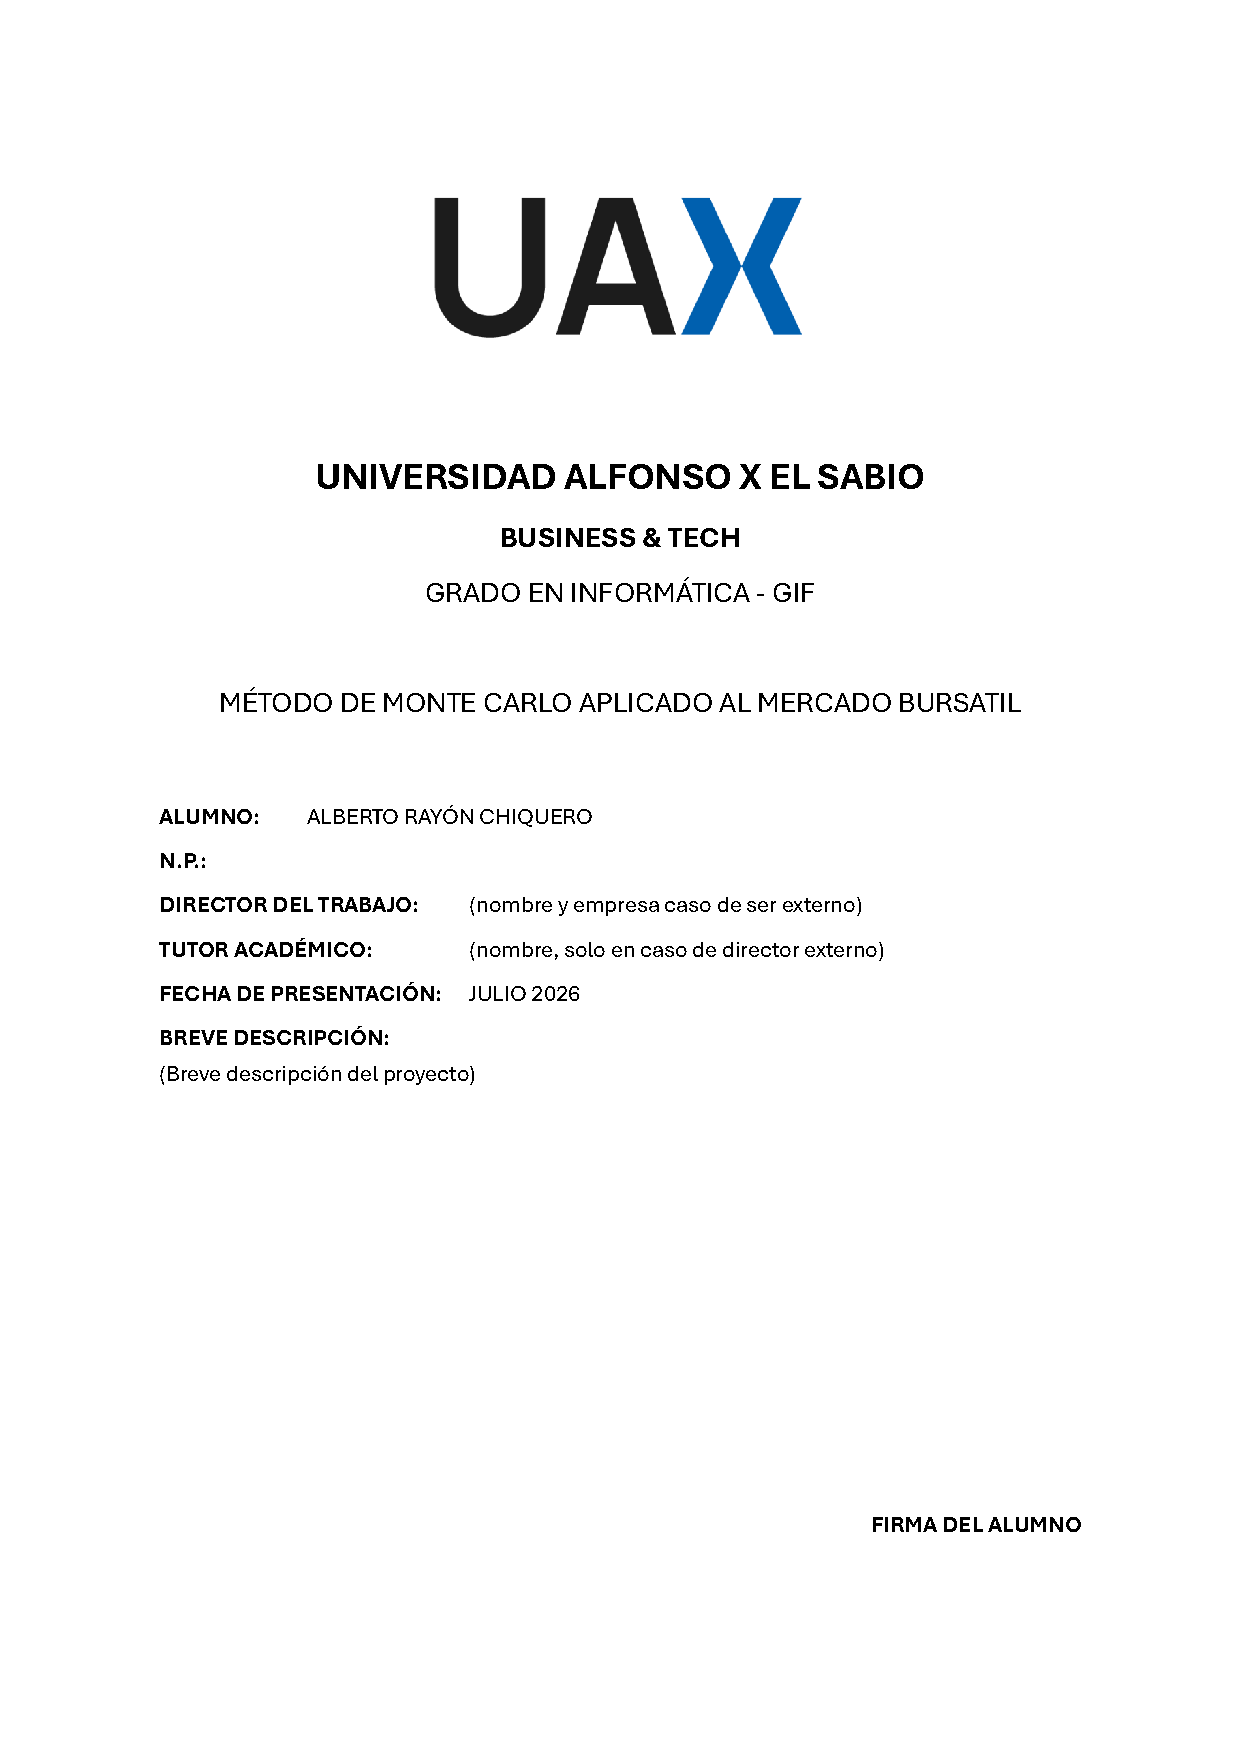
\includepdf{Hoja 1.pdf}

%\begin{titlepage}

%\centering



 

%\vspace*{1cm}

%{\bfseries\LARGE UNIVERSIDAD ALFONSO X EL SABIO \par}

%\vspace*{0.5cm}

%{\bfseries\Large BUSINESS \& TECH \par}

%\vspace*{0.5cm}

%{\bfseries\Large GRADO EN INFORMÁTICA \par}

%\vspace*{0.5cm}

%{\bfseries\Large (GIF) \par}

%\vspace*{1.5cm}

%\begin{figure}[h]

%\centering   

%\includegraphics[scale=4]%{logos_universidad/uax.pdf}
%   \label{fig:my_label}
%\end{figure}

%\vspace*{2cm}

%{\bfseries\Large TRABAJO FIN DE GRADO \par}

%\vspace*{1.5cm}

%{\normalfont\Large TITULO \par}

%\vspace*{5cm}
%{\bfseries\large Alberto Rayón Chiquero %\par}

%\vspace*{1cm}

%{\bfseries\large Julio 2026 \par}

%\end{titlepage}

 

%%%%%%%%%%%%%%%%%%%%%%%%%%%%% COMIENZA EL DOCUMENTO AQUI

%%%%CITAR: \cite{tipler2021fisica} 

%\newpage

%\thispagestyle{empty}

%\begin{center}

%\begin{figure}[H]

%\centering

%
\includegraphics[scale=0.1]{logos_universidad/uax.pdf}

%\end{figure}

%\vspace*{-1cm}

%\begin{figure}[h]

%\centering   

%\includegraphics[scale=3]%{logos_universidad/uax.pdf}
%   \label{fig:my_label}
%\end{figure}


%{\bfseries\Large UNIVERSIDAD ALFONSO X EL SABIO\par}

%\vspace*{0.5cm}

%{\bfseries\large BUSINESS \& TECH \par}

%\vspace*{0.5cm}

%{\scshape\large GRADO EN INFORMÁTICA - GIF \par}

%\vspace*{1.5cm}

%{\scshape\large TITULO \par}


%\end{center}

%\vspace*{1.5cm}

%{\textbf{ALUMNO:} ALBERTO RAYÓN CHIQUERO %\par}

%\vspace*{0.5cm}

%{\textbf{N.P:} \par}

%\vspace*{0.5cm}

%{\textbf{DIRECTOR DEL TRABAJO:} \par}

%\vspace*{0.5cm}

%{\textbf{FECHA DE PRESENTACIÓN:} \par}

%\vspace*{0.5cm}

%{\textbf{BREVE DESCRIPCIÓN:} \par}

%\vspace*{0.5cm}

%DESCRIPCIÓN

%\vspace*{5.5cm}
%\hspace*{10cm}
%{\textbf{FIRMA DEL ALUMNO} \par}

%\newpage{\ }

%\thispagestyle{empty}



%\includepdf{certificadotutores2.pdf}


 

\newpage{\ }

\thispagestyle{empty}

%\section*{Resumen}
 

\newpage{\ }

\thispagestyle{empty}

\section*{Palabras clave}

ejemplo palabra clave.


\newpage{\ }

\thispagestyle{empty}

\tableofcontents

\newpage

%%%%%%%%% MARCO DE PAGINA

\pagestyle{fancy}

\fancyhead[L]{
\includegraphics[scale=0.04]{logos_universidad/logo_UAX_png.png}}

\setcounter{page}{1}

\section{Introducción}

En el presente trabajo de fin de grado, vamos a abordar la necesidad de realizar el análisis de la evolución temporal del mercado bursatil, utilizando el método de Monte Carlo y simulaciones. Por último analizaremos los resultados obtenidos. \\ \\

Es un tema de especial interés ya que la economía mundial depende en gran medida de estos mercados y conocer y entenderlos bien es un tema importante. Para poder entenderlos mejor vamos a realizar un estudio detallado utilizando Movimiento Browniano Geométrico, para ello vamos a explicar el por qué de utilizar este tipo de movimiento (ya que se usa para definir el movimiento de las moléculas originalmente), una vez veamos la expresión del movimiento, vamos a utilizar el método de Monte Carlo para darle la ''aleatoriedad'' necesaria. \\ \\

Vamos a centrarnos en tres indices muy conocidos como son el IBEX 35 para representar los índices bursátiles de referencia de la bolsa española, el S\&P 500, para representar los índices bursátiles de referencia de Estados Unidos y el FTSE All-World, para representar los índices bursátiles más importantes a nivel mundial. Con estos indices podremos hacernos una idea de la evolución del mercado bursátil a nivel español y a nivel mundial. \\ \\


Con todos los datos generados, realizaremos la simulación usando la computación, con esta simulación vamos a ver la evolución temporal de los activos para posteriormente analizarlos. Para que los datos sean más exactos y ajustar la simulación, utilizaremos datos históricos para ciertos parámetros. \\ \\

Por último, representaremos los datos gráficamente y los analizaremos, obteniendo así diversas conclusiones.

\newpage

\section{Marco teórico}
\subsection{Movimiento browniano geométrico}

El uso del Movimiento browniano en física (teorizado en 1905 por Albert Einstein), define el movimiento errático de los átomos y moléculas, y estos movimientos son erráticos por el hecho de choques entre moléculas al azar (entre otras contribuciones) \cite{antonio2013movimiento} de aquí la similitud con el mercado bursatil, ya que en mercado se mueve de forma errática debido a los "choques" de noticias, resultados empresariales, decisiones de inversores, etc. \\

Además, este movimiento es crece de forma proporcional a su tamaño y es multiplicativo (no aditivo). \\

Esta movimiento tiene limitaciones \cite{joshi2003concepts}

\begin{itemize}
 \item Suponemos una volatilidad fija, cuando en la práctica puede ser variable.
 \item Asume que la "aleatoriedad" sigue una distribución normal, pero en la realidad puede haber cambios bruscos.
 \item No tiene en cuenta datos históricos (no tiene en cuenta tendencias históricas)
  \item El modelo es tiene una distribución suave y continua, en realidad los mercados pueden tener "picos".


\end{itemize} 

Vamos a desarrollar las expresiones matemáticas del movimiento browniano geométrico que usaremos posteriormente para la simulación. \\

Partiendo de la ecuación diferencial del movimiento browniano geométrico:


\begin{equation}
 dS_{t} =S_{t} \left (  \mu dt + \sigma  dW_{t} \right ) \to  \frac{dS_{t}}{S_{t}} = \mu dt + \sigma dW_{t}
\end{equation}

Siendo:

\begin{equation*}
\begin{matrix}
 S_{t} \;\; \textrm{Precio del activo} \;\;\;\;\;\;\;\;\;\;\;\;\;\;\;\;\;\;\;\;\;\;\;\;\;\;\;\;\;\;\;\;\;\;\;\;\;\;\;\; \\
 \mu \;\; \textrm{Rendimiento medio} \;\;\;\;\;\;\;\;\;\;\;\;\;\;\;\;\;\;\;\;\;\;\;\;\;\;\;\;\;\;\;\;\;\;\;\;\;\\
 \sigma \;\; \textrm{Volartilidad} \;\;\;\;\;\;\;\;\;\;\;\;\;\;\;\;\;\;\;\;\;\;\;\;\;\;\;\;\;\;\;\;\;\;\;\;\;\;\;\;\;\;\;\;\;\;\;\;\;\\
 t \;\; \textrm{Tiempo} \;\;\;\;\;\;\;\;\;\;\;\;\;\;\;\;\;\;\;\;\;\;\;\;\;\;\;\;\;\;\;\;\;\;\;\;\;\;\;\;\;\;\;\;\;\;\;\;\;\;\;\;\;\;\;\; \\
 W_{t} \;\; \textrm{Termino aleatorio (movimiento browniano)}
\end{matrix}
\end{equation*}

Para resolverlo, discretizámos los valores y aplicamos incrementos relativos (ya que $dS_{t}$ es proporcional de $S_{t}$)
\begin{equation}
\Delta S_{t} = S_{t} - S_{t+ \Delta t} \to S_{t+ \Delta t} = \Delta S_{t} + S_{t}\xrightarrow{\textrm{Dividimos todo por} \; S_{t}} \frac{S_{t+ \Delta t}}{S_{t}} = 1+\frac{\Delta S_{t}}{S_{t}}
\end{equation}

Tomando logaritmo natural y haciendo expansión de Taylor a orden 2 de $ 1+\frac{\Delta S_{t}}{S_{t}} $, la razón de quedarnos a orden 2 es porque $\left ( dW \right )^{2} \sim dt$ y no podemos quedarnos a orden 1 únicamente, por lo tanto, nos queda:

\begin{equation}
\ln \left (  \frac{S_{t+ \Delta t}}{S_{t}} \right ) = \ln \left ( 1+\frac{\Delta S_{t}}{S_{t}} \right ) \xrightarrow{\frac{\Delta S_{t}}{S_{t}}=x} \ln (1+x) \xrightarrow{\textrm{Aplicando Taylor hasta 2º orden  en x=0}} \ln(1+x) \approx  x- \frac{1}{2} x^{2}
\end{equation}

Por lo tanto, quitando el cambio $\frac{\Delta S_{t}}{S_{t}}=x$,  nos queda:

\begin{equation}
\ln \left (  \frac{S_{t+ \Delta t}}{S_{t}} \right ) = \ln \left ( 1+\frac{\Delta S_{t}}{S_{t}} \right ) \approx  \frac{\Delta S_{t}}{S_{t}} - \frac{1}{2} \left (  \frac{\Delta S_{t}}{S_{t}} \right )^{2}
\end{equation}

Sustituyendo en la expresión principal (discretizando), nos queda:
\begin{equation}
\ln \left (  \frac{S_{t+ \Delta t}}{S_{t}} \right ) \approx  \frac{\Delta S_{t}}{S_{t}} - \frac{1}{2} \left (  \frac{\Delta S_{t}}{S_{t}} \right )^{2} = \mu \Delta t + \sigma \Delta W_{t} - \frac{1}{2} \underset{    \mu^2 \Delta t^2 + \sigma^2 \Delta W_{t}^2 + 2  \mu \Delta t \sigma \Delta W_{t}       }{\underbrace{\left ( \mu \Delta t + \sigma \Delta W_{t} \right )^2}}
\end{equation}

Tomando las propiedades:

\begin{equation}
\begin{matrix}
\left ( \Delta t \right )^2 \to 0 \;\;\;\;\;\;\;\;\;\;\;\;\;\;\;\;\;\;\;\;\;\;\;\;\;\;\;\;\;\;\;\;\;\;\;\;\;\;\;\;\;\;\;\;\;\;\;\;\;\;\;\;\;\;\\
\left ( \Delta W \right )^2 \sim \ \Delta t \xrightarrow{\textrm{por lo tanto}} \Delta W \Delta t \sim \Delta t ^{3/2} \to 0
\end{matrix}
\end{equation}


Tenemos que:

\begin{equation*}
\ln \left (  \frac{S_{t+ \Delta t}}{S_{t}} \right ) \approx \mu \Delta t + \sigma \Delta W_{t} - \frac{1}{2} \left (   \mu^2 \cancelto{0}{ \Delta t^2} + \sigma^2 \Delta W_{t}^2 + 2  \mu \sigma   \cancelto{0}{\Delta t \Delta W_{t}} \right ) = \mu \Delta t + \sigma \Delta W_{t} - \frac{1}{2} \sigma^2 \Delta W_{t}^2  
\end{equation*}
Tomando la aproximación como correcta:
\begin{equation}
\ln \left (  \frac{S_{t+ \Delta t}}{S_{t}} \right ) = \mu \Delta t + \sigma \Delta W_{t} - \frac{1}{2} \sigma^2 \Delta W_{t}^2
\end{equation}

Reordenando y quitando el logaritmo natural tomando exponenciales:

\begin{equation*}
\ln\left(\frac{S_{t+\Delta t}}{S_{t}}\right)
= \left(\mu - \frac{1}{2}\sigma^2\right)\Delta t + \sigma \Delta W_{t}
\end{equation*}
\begin{equation*}
\frac{S_{t+\Delta t}}{S_t}
= e^{\left[\left(\mu - \frac{1}{2}\sigma^2\right)\Delta t + \sigma \Delta W_{t} \right]}
\end{equation*}
\begin{equation}
S_{t+ \Delta t}
= S_{t} \; e^{  \left[\left(\mu - \frac{1}{2}\sigma^2\right)\Delta t + \sigma \Delta W_{t} \right]}
\end{equation}
Iterando la expresión, llegamos a la solución:

\begin{equation}
\boxed{S_{t} = S_{0} e^{\left[\left(\mu - \frac{1}{2}\sigma^2\right)t + \sigma W_{t}\right]}}
\end{equation}

Siendo 
\begin{equation*}
\begin{matrix}
 S_{t} \;\; \textrm{Precio del activo} \;\;\;\;\;\;\;\;\;\;\;\;\;\;\;\;\;\;\;\;\;\;\;\;\;\;\;\;\;\;\;\;\;\;\;\;\;\;\;\; \\
S_{0} \;\; \textrm{Precio del actual} \;\;\;\;\;\;\;\;\;\;\;\;\;\;\;\;\;\;\;\;\;\;\;\;\;\;\;\;\;\;\;\;\;\;\;\;\;\;\;\; \\
 \mu \;\; \textrm{Rendimiento medio} \;\;\;\;\;\;\;\;\;\;\;\;\;\;\;\;\;\;\;\;\;\;\;\;\;\;\;\;\;\;\;\;\;\;\;\;\;\\
 \sigma \;\; \textrm{Volartilidad} \;\;\;\;\;\;\;\;\;\;\;\;\;\;\;\;\;\;\;\;\;\;\;\;\;\;\;\;\;\;\;\;\;\;\;\;\;\;\;\;\;\;\;\;\;\;\;\;\;\\
 t \;\; \textrm{Tiempo} \;\;\;\;\;\;\;\;\;\;\;\;\;\;\;\;\;\;\;\;\;\;\;\;\;\;\;\;\;\;\;\;\;\;\;\;\;\;\;\;\;\;\;\;\;\;\;\;\;\;\;\;\;\;\;\; \\
 W_{t} \;\; \textrm{Termino aleatorio (movimiento browniano)}
\end{matrix}
\end{equation*}


\subsection{Método de Monte Carlo}

El método de Monte Carlo \cite{vega2012metodo} surge en los años 40, y fue desarrollado por Stanislaw Ulam y John von Neumann. Se desarrolló para resolver el estudio de la difusión de neutrones en reacciones nucleares, esto fue en el proyecto Manhattan, en el Laboratorio Nacional de Los Álamos durante la Segunda Guerra Mundial, en el desarrollo de la bomba atómica. \\ \\

En el proyecto Manhattan necesitaban resolver resolver el problema antes propuesto y era extremadamente complejo, ya que eran imposibles de calcular de forma exacta, por lo idearon un sistema de simulación aleatoria en lugar de buscar soluciones analíticas. Stanislaw Ulam mientras se recuperaba de una enfermedad, se puso a pensar y se dio cuenta que era más fácil simular diversos escenarios aleatorios y observar las combinaciones posibles que resolver el problema de forma exacta. El nombre lo propuso John von Neumann, al hacer referencia a la aleatoriedad con los juegos de azar, al igual que los juegos de casino, y aquí entra la asociación con el casino de Monte Carlo, de aquí su nombre. \\ \\

Actualmente, se utiliza como una técnica computacional estadística por su facilidad para ser implementado, y por su capacidad de resolución de problemas complejos sin solución exacta. Se usa en diversos campos como en física, en análisis de mercados bursatiles, inteligencia artificial, etc. 
 
\subsection{Generación de números aleatorios}

Los números aleatorios son números que pueden ser generados a partir de fuentes de aleatoriedad, generalmente, de naturaleza física y siguen reglas de las leyes del azar. Por otra parte, los números pseudo-aleatorios son los números que siguen un comportamiento similar a los de naturaleza aleatoria, pero que están limitados por un patrón, por lo general de naturaleza matemática, el cual hace que su comportamiento sea determinístico \cite{herrera2000numeros}. \\ \\

La generación de números aleatorios de calidad es fundamental, la mayotia de los números aleatorios actuales son casos especiales del generador Congruencial Lineal de Lehmer, en el cual se escogen 4 números enteros no negativos:
\begin{equation*}
\begin{matrix}
X_{0} \\
a \\
c\\
m
\end{matrix}
\to
\left\{\begin{matrix}
m > X_{0} ,m> a, m> c \\
X_{0},a,c,m \in \mathbb{N} \geq 0
\end{matrix}\right.
\end{equation*}
Cuya secuencia es: 
\begin{equation}
X_{i+1} = \left ( a X_{i} +c \right ) \textrm{mod} \;\; m
\end{equation}



\newpage

\section{Simulación}
dfg

\newpage
\section{Análisis de datos y conclusiones}
















ejemplo cita \cite{zapata2004metodo}


\newpage



\bibliographystyle{IEEEtran}
\bibliography{bibliografia.bib}

\end{document}